$subject$=Дополнительные главы \\ высшей математики
$date$=21.03.2025
$teacher$=Лекции Далевской О. П.

\begin{enumerate}[label=\arabic*$^\circ$]
    \setcounter{enumi}{3}
    \item $f(z)$ аналитична в $D \ (f : D \longrightarrow D^\prime)$, $f^\prime(z) \neq 0 \ \forall z \in D$. 
    Тогда $\exists g(w) = f^{-1}(z) \ (g : D^\prime \longrightarrow D)$ и $\forall z_0 \in D \ f^\prime_z (z_0) = \frac{1}{g^\prime_w (w_0)}$,
    где $w_0 = w(z)$

    \begin{MyProof}
        $f(z) = u(x, y) + i v(x, y)$

        Заметим, что $f^\prime(z) \neq 0 \Longleftrightarrow 
        \begin{vmatrix}\frac{\partial u}{\partial x} & \frac{\partial u}{\partial y} \\ \frac{\partial v}{\partial x} & \frac{\partial v}{\partial y}\end{vmatrix} = J \neq 0$

        Действительно, если якобиан равен 0, то $\frac{\partial u}{\partial x} \frac{\partial v}{\partial y} - \frac{\partial u}{\partial y} \frac{\partial v}{\partial x} = 0 \Longrightarrow 
        \frac{\partial u}{\partial x} \frac{\partial u}{\partial x} + \frac{\partial v}{\partial x} \frac{\partial v}{\partial x} = 0$. Аналогично $\frac{\partial u}{\partial y} \frac{\partial u}{\partial y} + \frac{\partial v}{\partial y} \frac{\partial v}{\partial y} = 0$

        Значит, $\frac{\partial u}{\partial x} = \frac{\partial v}{\partial x} = \frac{\partial u}{\partial y} = \frac{\partial v}{\partial y} = 0$ -- противоречие

        Если $J \neq 0$, то преобразование $f(z)$ приводит $(x, y)$ в $(u, v)$ взаимно однозначно. Тогда $\exists!$ решение
        \begin{cases}
            u = u(x, y) \\
            v = v(x, y)
        \end{cases}, то есть взаимно однозначно определены \begin{cases}
            x = x(u, v) \\
            y = y(u, v)
        \end{cases}

        Обозначим $g(w) = x(u, v) + i y(u, v)$

        Найдем $f^\prime_z(z_0) = \frac{1}{g^\prime_w(w_0)}$. 
        Рассмотрим отношение $\frac{\Delta z}{\Delta w} \underset{\Delta z \to 0}{\overset{\Delta w \to 0}{\longrightarrow}} 
        \lim_{\substack{\Delta w \to 0 \\ \Delta z \to 0}} \frac{\Delta z}{\Delta w} = \lim_{\substack{\Delta w \to 0 \\ \Delta z \to 0}} \frac{1}{\frac{\Delta w}{\Delta z}} = 
        \frac{1}{\lim_{\Delta z \to 0} \frac{\Delta w}{\Delta z}} = \frac{1}{f^\prime_z (z_0)} \Longrightarrow \lim_{\Delta w \to 0} \frac{\Delta z}{\Delta w} = g^\prime_w(w_0) = \frac{1}{f^\prime_z(z_0)}$ или $f^\prime_z(z_0) = \frac{1}{g^\prime_w(w_0)}$
    \end{MyProof}

    \item $f(z) = u(x, y) + i v(x, y)$ аналитична в $D$. Тогда $u(x, y), v(x, y)$ -- гармонические функции в $D$

    \begin{MyProof}
        Функция считается гармонической, если $\Delta u = 0$ (здесь $\Delta = \nabla^2$ -- лапласиан) $\Longleftrightarrow u_{xx} + u_{yy} = 0$
        
        \Lab
    \end{MyProof}

    \item Если $f(z) = u(x, y) + i v(x, y)$ аналитична в $D$ и известна $u(x, y)$ или $v(x, y)$, то $f(z)$ определяется однозначно с точностью до $\operatorname{const}$

    \begin{MyProof}
        Пусть известна $\RE f(z) = u(x, y)$. Нужно найти $v(x, y)$. По условию Коши-Римана $\int u(x, y), \int v(x, y)$ не зависят от пути
        (\Lab доказать, что $\int_{AB} dv$ не зависит от пути)

        $v(x, y) = \int_{(x_0, y_0)}^{(x, y)} dv(x, y) = \int_{(x_0, y_0)}^{(x, y)} v_x dx + v_y dy = \int_{(x_0, y_0)}^{(x, y)} (-u_y) dx + u_x dy$

        Интеграл будет найден с точностью до $\operatorname{const} = C(x_0, y_0)$
    \end{MyProof}

\end{enumerate}


\subsection{2.5. Конформные отображения}

Найдем геометрический смысл производной. Рассмотрим отображение $w = f(z) \ (w : D \longrightarrow G)$ -- дифференцируема в точке $z_0 \in D$ и $f^\prime(z_0) \neq 0$

\underline{Аргумент}: В области $D$ рассмотрим гладкую кривую $\gamma(t) = \varphi(t) + i\psi(t)$. Образ $\gamma(t)$ -- кривая $\sigma(t)$ в $G$

$\gamma(t)$ в окрестности некоторой точки $z_0$ гладкая, $\exists$ касательная с углом $\theta = \arg \gamma^\prime(t)$

$\sigma(t)$ в окрестности $w_0 = w(z_0)$ гладкая, $\exists$ касательная с углом $\theta^\prime = \arg \sigma^\prime(t)$

А $\sigma^\prime(t_0) = w^\prime (t_0) = f^\prime(z_0) \cdot \underset{z^\prime(t_0)}{\underbrace{\gamma^\prime(t_0)}}$

$\arg w^\prime(t_0) = \arg f^\prime (z_0) + \arg \gamma^\prime(t_0)$

$\theta^\prime = \arg f^\prime(z_0) + \theta$

$\theta^\prime - \theta = \arg f^\prime (z_0)$ -- поворот кривой $\gamma(t)$ вокруг $z_0$ на угол $\arg f^\prime(z_0)$ при отображении $w = f(z)$

% https://www.geogebra.org/calculator/kkfcrxt4

\begin{multicols}{2}
    \begin{center}
        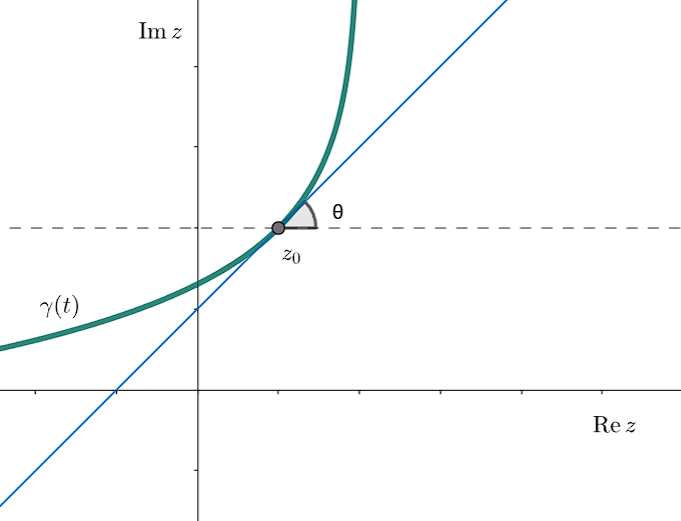
\includegraphics[height=5cm]{addchapters2/images/addchapters2_2025_03_21_1}

        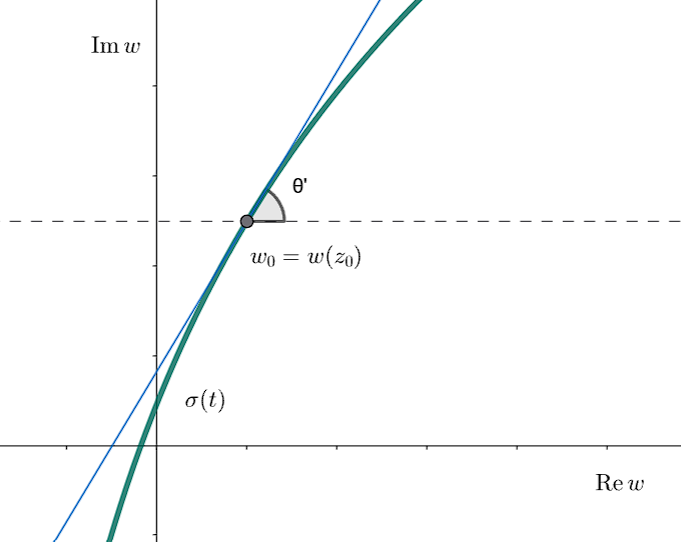
\includegraphics[height=5cm]{addchapters2/images/addchapters2_2025_03_21_2}
    \end{center}
\end{multicols}

\mediumvspace

\underline{Модуль}: $w = f(z)$ -- дифференцируема $\Longleftrightarrow \Delta w = f^\prime(z_0) \Delta z + o(\Delta z)$

Рассмотрим $\lim_{\Delta z \to 0} \left|\frac{\Delta w}{\Delta z}\right| = |f^\prime(z_0)| \Longrightarrow |\Delta w| = |f^\prime(z_0)| \cdot |\Delta z| + o(|\Delta z|)$

Рассмотрим малый контур $|\Delta z| = |z - z_0| = \rho$. Тогда $|\Delta w| = |w(z) - w(z_0)| = |f^\prime(z)| \rho + o(\rho)$

Таким образом $w(z)$ растягивает круг $|z - z_0| = \rho$ в $|f^\prime(z_0)|$ раз с точностью до малых высших порядков

\mediumvspace

\hypertarget{geometrical_meaning_of_derivative}{}

Итак, $w = f(z)$ в точке $z_0$ поворачивает точку у окрестности на угол $\alpha = \arg f^\prime(z_0)$ и растягивает отрезки $[z_0, z]$ в $k = |f^\prime(z_0)|$ раз

\hypertarget{conformal_map}{}

\Def Конформное отображение -- отображение $w(z)$, сохраняющее углы (между образами и прообразами) и постоянство растяжений

\begin{MyTheorem}
    \Ths Условия конформности: \begin{cases}\text{дифференцируемость} \\ \text{однолистность} \\ f^\prime(z) \neq 0 \text{ в } D\end{cases} $\Longleftrightarrow$ конформно
\end{MyTheorem}

\Ex $w = az + b$

\Mems Геометрический смысл линейного отображения: $b$ - перенос $z = 0$ в точку $z = b$; $a = |a| e^{i\varphi}$, тогда 
$|a|$ - коэффициент растяжения, $\varphi$ - угол поворота

Заметим, $w^\prime = (az + b)^\prime = a$, тогда $k = |w^\prime(z_0)| = |a|$, $\varphi = \arg w^\prime(z_0) = \arg a$

\Lab Проверить, что $w = z^2$ не конформное отображение, найдя $w^\prime(z_0)$

\section{3. Интеграл по комплексной переменной}

\subsection{3.1. Определения}

\smallvspace

\hypertarget{complex_integral}{}

В $\Complex$ задана кусочно-гладкая кривая $K$ (с концами в точках $M$ и $N$) параметрическими уравнениями: 

\begin{cases}
    x = \varphi(t) & \qquad t \in [\alpha, \beta] \subset \Real \\
    y = \psi(t) & \qquad \varphi, \psi \text{ -- } \Real \text{-функции} \\
\end{cases}

Тогда $z(t) = \varphi(t) + i \psi(t)$ - задание $K$ в $\Complex$. Введем отображение $w = f(z)$, действующее на $K$

Определим интегральные суммы:

\begin{enumerate}
    \item Дробление отрезка $MN$ на частичные дуги: $M = z_0, z_1, \dots, z_{n - 1}, z_n = N$

    Тогда $\alpha = t_0, t_1, \dots, t_{n - 1}, t_n = \beta$

    \item Выбор средних точек в отрезках кривой $\zeta_i = (\xi_i, \eta_i)$

    \item Сопоставим интегральную сумму $\sigma_n = \sum_{i = 1}^n f(\zeta_i) \Delta z_i$

    \item Интегралом от $w = f(z)$ по кривой $K$ называется $\lim_{\substack{n \to \infty \\ \tau = \max \Delta z_i \to 0}} \sigma_n = 
    \int_K f(z) dz$, если он существует, конечен и не зависит от способа разбиения, выбора средних точек и т. д.
\end{enumerate}

При этом интеграл можно представить как $\lim_{n \to \infty} \sigma_n = \lim_{n \to \infty} \sum_{i = 1}^n f(\zeta_i) \Delta z_i = 
\lim_{n \to \infty} \sum_{i = 1}^n f(\xi_i, \eta_i) (\Delta x_i + i \Delta y_i) = 
\lim_{n \to \infty} \sum_{i = 1}^n (u(\xi_i, \eta_i) + i v(\xi_i, \eta_i)) (\Delta x_i + i \Delta y_i) = 
\lim_{n \to \infty} \sum_{i = 1}^n (u_i \Delta x_i - v_i \Delta y_i) + i \lim_{n \to \infty} \sum_{i = 1}^n (u_i \Delta y_i + v_i \Delta x_i) =
\int_K udx - vdy + i \int_K udy + vdx$

\Nota Мы свели $\Complex$-интеграл к двум криволинейным $\Real$-интегралам, все свойства интегралов сохраняются

\Ex $\int_{\gamma = [0; 1 + i]} \overline{z} dz = \int_\gamma (x - iy) (dx + idy) = 
\int_\gamma xdx + ydy + i \int_\gamma xdy - ydx = 2 \int_0^1 xdx = 1$
